%!TEX root = main.tex

\section{Adaptive exploration with a three-level disclosure policy}
\label{sec:3level}

The two-level policy from the previous section implements the explore-then-exploit paradigm using a basic design with parallel full-disclosure paths. The next challenge is to implement \emph{adaptive exploration}, and go below the $T^{2/3}$ barrier. We accomplish this using a construction that adds a middle level to the info-graph. This construction also provides intuition for the main result, the multi-level construction presented in the next section. For simplicity, we assume $K=2$ arms.

\begin{figure}[t]
\centering
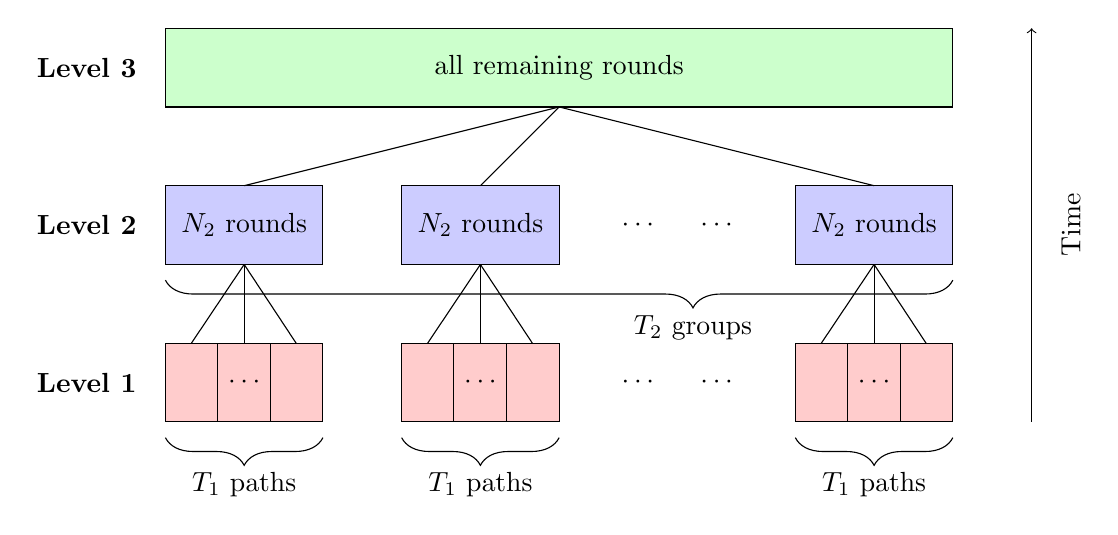
\begin{tikzpicture}
 \filldraw[fill=green!20!white]
 (0,4)--(10,4)--(10,5)--(0,5)--cycle;
 \foreach \x in {0,3,8}
 {
 \filldraw[fill=blue!20!white]
 (\x+0,2)--(\x+2,2)--(\x+2,3)--(\x+0,3)--cycle;
 \draw (\x+1,3)--(5,4);
 \filldraw[fill=red!20!white]
 (\x+0,0)--(\x+2,0)--(\x+2,1)--(\x+0,1)--cycle;
 \draw (\x+1,1)--(\x+1,2);
 \draw(\x+0.33,1)--(\x+1,2);
 \draw(\x+1.66,1)--(\x+1,2);
 %\draw(\x+1.4,1)--(\x+1,2);
 %\draw(\x+1.8,1)--(\x+1,2);
 \draw(\x+0.66,0)--(\x+0.66,1);
 \draw(\x+1.33,0)--(\x+1.33,1);
% \draw (\x+1.2,0)--(\x+1.2,1);
 %\draw(\x+1.6,0)--(\x+1.6,1);
 \node at(\x+1,2.5){$N_2$ rounds};
 \node at(\x+0.33, 0.5){$\GdT$};
 %\node at(\x+0.6, 0.5){$\cdot$};
 \node at(\x+1.0, 0.5){$\cdots$};
 %\node at(\x+1.4, 0.5){$\cdot$};
 \node at(\x+1.66, 0.5){$\GdT$};
 %\node at(\x+1,0.5){$T_1 \cdot \GdT$};
 \draw [decorate,decoration={brace,amplitude=10pt},xshift=0pt,yshift=0pt] (\x+2,-0.2) -- (\x+0,-0.2) node [black,midway,yshift=-0.6cm] {$T_1$ paths};
 }
  \node at(5,4.5){all remaining rounds};
  \node at (6,0.5){$\cdots$};
  \node at (7,0.5){$\cdots$};
  \node at (6,2.5){$\cdots$};
  \node at (7,2.5){$\cdots$};
  \node at(-1,0.5){\textbf{Level 1}};
  \node at(-1,2.5){\textbf{Level 2}};
  \node at(-1,4.5){\textbf{Level 3}};
  \draw[->] (11,0)--(11,5);
  \node at(11.5,2.5)[ rotate=90]{Time};

  \draw [decorate,decoration={brace,amplitude=10pt,aspect=0.33},xshift=0pt,yshift=0pt] (10,1.8) -- (0,1.8) node [black,pos=0.33,xshift = 0cm,yshift=-0.6cm] {$T_2$ groups};

\end{tikzpicture}
\caption{Info-graph for the three-level policy. Each red box in level 1 corresponds to $T_1$ full-disclosure paths of length $\GdT$ each.}
\label{fig:3level}
\end{figure}


The new policy, called the \emph{three-level policy}, is as follows
 (see Figure~\ref{fig:3level}).

\begin{construction}
The info-graph consists of three levels: the first two correspond to \emph{exploration}, and the third implements \emph{exploitation}. Like in the two-level policy, the first level consists of multiple full-disclosure paths of length $\fdpL$ each, and each agent $t$ in the exploitation level sees full history from exploration. The middle layer is what ensures adaptive exploration. It consists of $T_2$ disjoint subsets of $N_2$ agents each, called \emph{second-level groups}. Each second-level group $S$ has the following property:
\begin{align}\label{eq:group-defn}
\text{all nodes in $S$ are connected to the same nodes outside of $S$, but not to one another.}
\end{align}

The full-disclosure paths in the first level are also split into $T_2$ disjoint subsets, called \emph{first-level groups}. Each first-level group consists of $T_1$ full-disclosure paths, for the total of $T_1\cdot T_2\cdot \fdpL$ rounds in the first layer. There is a 1-1 correspondence between first-level groups $S_1$ and second-level groups $S_2$, whereby each agent $t\in S_2$ observes the full history from the corresponding group $S_1$. More formally, agent $t$ is connected to the last node of each full-disclosure path in $S_1$. In other words, this agent receives message
    $m_t = \SubH{V(S_1)}$,
where $V(S_1)$ is the set of all rounds in $S_1$. 
\end{construction}

\begin{theorem}
\label{thm:3level}
For two arms, the three-level policy
achieves regret
\[ \reg(T) \leq O\left( T^{4/7}\, \log T \right).\]
This is achieved with parameters
    $T_1 = T^{4/7}\log^{-1/7}(T)$,
    $T_2 = 2^{10}\log(T)$, and
    $N_2 = T^{6/7}\log^{-5/7}(T)$.
\end{theorem}

\ascomment{Parameter change: what I call $T_2$ used to be $S$, and what I call $N_2$ used to be $T_2$.}

\ascomment{stopped here.}

They main idea for the 3-level policy is that it inserts the second level as an additional ``checkpoint'' to induce more adaptivity in the exploration. \niedit{While the first level ensures that the agents explore both arms, the better arm can only be discovered if the gap in their rewards $|\mu_1-\mu_2|$ is sufficiently high.  When this gap is small (that is, when $|\mu_1 - \mu_2| < \tilde{O}(1/\sqrt{T_1})$), we argue that the second level will continue to explore both arms.  Here we use the anti-concentration bound to show each arm is ``lucky'' in at least one first level group (that is, for some first level group, its empirical mean is significantly larger than its mean whereas the other arm's empirical mean is significantly smaller than its mean).  Therefore, the corresponding second level group will explore the lucky arm, giving the third level refined estimates of each arm's mean.}  In the third level, agents will pull the best arm unless $|\mu_1-\mu_2|$ is much smaller than $\tilde{O}(1/\sqrt{T_2})$, in which case pulling either arm will
incur small regret. The formal guarantee of the policy is the
following. \nicomment{I'm a little confused why this works while simply growing the first level doesn't work; wouldn't the first level where the arm is ``lucky'' explore it more if it had more time?}








\iffalse
In the proof, we need not only the concentration argument as the
2-level recommendation policy, but also the anti-concentration
argument to show that agents explore more in the second round if
$\mu_1-\mu_2$ is not too big.

Set $T_1 = T^{4/7}\log^{-1/7}(T)$ and $T_2 =
T^{6/7}\log^{-5/7}(T)$. The first level has $S = 2^{10}\log(T)$ groups
of agents. Each group runs $T_1$ \ALGG of $T_G$ rounds in
parallel. The second level also has $S$ groups of agents. Each group
has $T_2$ agents and they observe the history of corresponding group
in the first level. All the rest agents are in the third level and
they observe the entire history of the first two levels.  See also
Figure \ref{fig:3level} for a graphical view of the information flow.



Here we give some intuition about how the 3-level recommendation
policy works. The main idea is to do the exploration more
adaptively. In the first level, agents explore both arms. In the
second level, agents will pull the best arm when $\mu_1 - \mu_2$ is
large ($\tilde{\Omega}(1/\sqrt{T_1})$). Otherwise agents will explore
both arms more. In the third level, agents will pull the best arm
unless $\mu_1-\mu_2$ is much smaller ($\tilde{O}(1/\sqrt{T_2})$). In
the proof, we need not only the concentration argument as the 2-level
recommendation policy, but also the anti-concentration argument to
show that agents explore more in the second round if $\mu_1-\mu_2$ is
not too big.
\fi




\subsection{Events}
We will first establish four events that together occur
with probability at least $1 - O(1/T)$. The first event says that
every group of \ALGG runs in the first level ensures that each arm $a$
is pulled at least $\Omega(T_1)$ times. The following lemma can
derived from combining Lemma~\ref{lem:t1runs} and union bound.

\begin{lemma}[Concentration of first-level number of pulls.]\label{3levelw1}
  Let $W_1$ be the event that for all groups $s\in [S]$ and arms
  $a\in \{1, 2\}$, the number of arm $a$ pulls in the $s$-th
  first-level group is in the range of
  $$
  \left[\fdpN  T_1- \GdT \sqrt{T_1\log(T)}, \fdpN  T_1 + \GdT \sqrt{T_1\log(T)}\right],
  $$
  where $\fdpN $ is the expected number of arm $a$ pulls in a $\ALGG$ run
  of length $\GdT$. Then $\Pr[W_1] \geq 1- \frac{4S}{T^2}$.
\end{lemma}


The next two events are about the distribution of the mean rewards in
the first level. To state the events, it will be useful to think of a
hypothetical reward tape $\cT^1_{s, a}$ of length $T$ for each
group $s$ and arm $a$, with each cell independently sampled from
$\cD_a$.  The tape encodes rewards as follows: the $j$-th time arm $a$
is chosen by the group $s$ in the first level, its reward is taken
from the $j$-th cell in this arm's tape. The following result
characterizes the concentration of the mean rewards among all
consecutive pulls among all such tapes, which follows from Chernoff
bound and union bound.

\begin{lemma}[Concentration of empirical means in the first level]\label{3levelw2}
  For any $t_1, t_2\in [T]$ such that $t_1 < t_2$, $s\in [S]$, and
  $a\in \{1,2\}$, let $W_2^{s,a,t_1,t_2}$ be the event that the mean
  among the cells indexed by $t_1, (t_1+1), \ldots, t_2$ in the tape
  $\cT^1_{a, s}$ is at most $\sqrt{\frac{2\log(T)}{t_2-t_1+1}}$ away
  from $\mu_a$.  Let $W_2$ be the intersection of all these events
  (i.e.  $W_2 = \bigcap_{a,s,t_1,t_2} W_2^{s,a,t_1,t_2}$). Then
  \[
    \Pr[W_2] \geq 1- \frac{4S}{T^2}.
  \]
\end{lemma}

Our policy also relies on the anti-concentration of the empirical
means in the first round. We show that for each arm $a\in \{1, 2\}$,
there exists a group $s_a$ such that the empirical mean of $a$ is
slightly above $\mu_a$, while the other arm $(3 - a)$ has empirical
mean slightly below $\mu_{(3-a)}$. This event is crucial for inducing
agents in the second level to explore both arms when the their
mean rewards are indistinguishable after the first level.


\begin{lemma}[Co-occurence of high and low deviations]\label{3levelw4}
  For any group $s\in [S]$, any arm $a$, let $\tilde\mu_{a,s}$ be the
  empirical mean of the first $\fdpN  T_1$ cells in tape $\cT^1_{a, s}$.
  Let $W_4^{s,a,\text{high}}$ be the event
  $\tilde\mu_{a, s} \geq \mu_a + 1/\sqrt{\fdpN  T_1}$ and let
  $W_4^{s,a,\text{low}}$ be the event that
  $\tilde\mu_{a, s} \leq \mu_a - 1/\sqrt{\fdpN  T_1}$.  Let $W_4$ be the
  event that for every $a\in \{1, 2\}$, there exists a group
  $s_a\in [S]$ in the first level such that both $W_4^{s_a,a,\text{high}}$
  and $W_4^{s_a,3-a,\text{low}}$ occur. Then
  \[
    \Pr[W_4]\geq 1 -2 /T.
  \]
\end{lemma}




Lastly, we will condition on the event that the empirical means of
both arms are concentrated around their true means in any prefix of
their pulls. This guarantees that the policy obtains an accurate
estimate of rewards for both arms after aggregating all the data in
the first two levels.
% We will again state the event using a hypothetical reward tape
% $\cT^2_a$ for each arm $a$: the $j$-th time arm $a$ is chosen in the
% two levels, its reward is taken from the $j$-th cell in $\cT^2_a$.


\swcomment{might want to swap out $W_3$ and $W_4$} \nicomment{yes please!}

\begin{lemma}[Concentration of empirical means in the first two
  levels]\label{3levelw3}
  With probability at least $1 - \frac{4}{T^3}$, the following event
  $W_3$ holds: for all $a\in \{1, 2\}$ and $m \in [N_{T, a}]$, the
  empirical means of the first $t$ \nicomment{what is $t$ here; you mean $m$? in which case please replace $m$ with $t$ in the conditioning and bound} arm $a$ pulls is at most
  $\sqrt{\frac{2\log(T)}{m}}$ away from $\mu_a$, where $N_{T, a}$ is
  the total number of arm $a$ pulls by the end of $T$ rounds.
\end{lemma}




Let $W = \bigcap_{i=1}^4 W_i$ be the intersection of all 4
events.  By union bound, $W$ occurs with probability $1-O(1/T)$. Note
that expected regret conditioned on $W$ not occuring is at most
$O(1/T) \cdot T = O(1)$, so it suffices to bound the regret conditioned on $W$.

\subsection{Case Analysis}

We now proceed to bound the regret conditioned on the four
events defined above. Without loss of generality, we assume
$\mu_1 \geq \mu_2$ as the recommendation policy is symmetric to both
arms. We break down the regret analysis into four cases on the scale
of the gap parameter $\Delta = (\mu_1-\mu_2)$.


We will start with the simplest case where the gap is smaller than
$\tilde O(\sqrt{1/T_2}) = \tilde O(1/T^{3/7})$, then the regret is
trivially bounded by $\tilde O(T^{4/7})$.

\begin{claim}[Negligible gap case]
  Suppose $\Delta \leq 3\sqrt{\frac{2\log(T)}{T_2}}$,
  $\reg(T)\leq O(T^{4/7} \log^{6/7}(T))$.
\end{claim}

Another simple case is when $\Delta$ is sufficiently large, so that
the data collected in any single first-level group can distinguish the
two arms. The proof essentially follows from the event $W_1$
that both arms are explored sufficient many times in level 1, and the
empirical rewards in the first two levels concentrate around their
true means.

\begin{lemma}[Large gap case]\label{3levelbigcase}
  Suppose
  $\Delta \geq 2\left(\sqrt{\frac{4\log(T)}{\fdpN[1]T_1}} +
    \sqrt{\frac{4\log(T)}{\fdpN[2]T_1}}\right)$, then all agents in the
  second and third levels pull arm 1.
\end{lemma}


There are two more intermediate cases. In the \emph{medium gap} case,
the gap is smaller than $\tilde O(\sqrt{1/T_1})$, but bigger than
$\tilde \Omega(\sqrt{1/(S\, T_1)})$. Then the data collected in any
single group from the first level no longer suffices to distinguish
the two arms. However, we show that as the policy aggregates the
history from all $S$ groups at the end of the second level, the data
will enable all third-level agents to correctly identify the arm 1 as
the better arm (even though one of the arms may not be pulled at all
in the second level).

\begin{lemma}[Medium gap case]\label{3levelmedium}
  All agents pull arm 1 in the third level, when $\Delta$ satisfies
  \[
  \Delta\in \left[
   2\left(\sqrt{\frac{4\log(T)}{S\fdpN[1]T_1}} +
    \sqrt{\frac{4\log(T)}{S\fdpN[2]T_1}}\right),
 2\left(\sqrt{\frac{4\log(T)}{\fdpN[1]T_1}} +
        \sqrt{\frac{4\log(T)}{\fdpN[2]T_1}}\right),
    \right)
  \]
\end{lemma}


Finally, consider the \emph{small gap} case where $\Delta$ is between
$\tilde\Omega(\sqrt{1/T_2})$ and $\tilde O(\sqrt{1/(S T_1))})$. This
is more challenging since even aggregating the data from all $S$
groups in the first level is not sufficient for correctly
distinguishing the two arms. Thus, we need to ensure that both arms
will continue to be pulled in the second level. To achieve this, we
will nicely leverage the event of $W_4$, which has the implication
that each arm $a$ has a ``lucky'' group $s_a$ in the first level,
for which its empirical mean is slightly higher than $\mu_a$, while
the other arm is slightly lower than $\mu_{(3-a)}$. Since the
deviations are in the order of $\Omega(\sqrt{1/T_1})$, and Assumption~\ref{ass:embehave} guarantees the estimates are also within $\Omega(\sqrt{1/T_1})$ of the empirical means, the sub-history
from this ``lucky'' group will yield estimates such that
$\hat \mu_a^t > \hat \mu_{(3-a)}^t$, and so any second-level agent in
group $s_a$ will pull arm $a$.  As a result, we guarantee both arms
will be pulled at least $T_2$ times in the second level, which in turn
gives the following guarantee.


\begin{lemma}[Small gap case]\label{3levelsmallcase}
  All agents pull arm 1 in the third level, when $\Delta$ satisfies
  \[
    \Delta\in \left( 3\sqrt{\frac{2\log(T)}{T_2}},
      2\left(\sqrt{\frac{4\log(T)}{S \fdpN[1]T_1}} +
        \sqrt{\frac{4\log(T)}{S \fdpN[2]T_1}}\right) \right)
  \]
\end{lemma}


\paragraph{Wrapping up: proof of \Cref{thm:3level}. } In negligible
gap case, the stated regret bound holds regardless of the sequence of
chosen arms. In the large gap case, the regret only comes from the
first level, which is bounded
by $S \GdT T_1 = O(T^{4/7} \log^{6/7}(T))$. In the intermediate cases of
both medium and small gaps, it suffices to bound the regret from the
first and second levels, so
\[
\reg(T) \leq (S \GdT T_1 + S T_2) \cdot 2\left(\sqrt{\frac{4\log(T)}{\fdpN[1]T_1}}
+ \sqrt{\frac{4\log(T)}{\fdpN[2]T_1}}\right) = O(T^{4/7} \log^{6/7}(T)).
\]
Therefore, we obtain the stated regret bound in all cases.




\OMIT{
\begin{proof}
Wlog we assume $\mu_1 \geq \mu_2$ as the recommendation policy is symmetric to both arms. We do a case analysis based on $\mu_1-\mu_2$.

Before we start with the case analysis, we first define several clean events and show that the intersection of them happens with high probability.

\begin{itemize}

\item \textbf{Concentration of the number of arm $a$ pulls in the first level:}
\OMIT{By Lemma \ref{lem:greedy}, we know $\GdP \leq \fdpN  \leq \GdT$. For the $s$-th first-level group, define $W_1^{a,s}$ to be the event that the number of arm $a$ pulls in the $s$-th first-level group is between $\fdpN  T_1- \GdT \sqrt{T_1\log(T)}$ and $\fdpN  T_1 + \GdT \sqrt{T_1\log(T)}$. By Chernoff bound,}
For the $s$-th first-level group, define $W_1^{a,s}$ to be the event
that the number of arm $a$ pulls in the $s$-th first-level group is
between $\fdpN  T_1- \GdT \sqrt{T_1\log(T)}$ and
$\fdpN  T_1 + \GdT \sqrt{T_1\log(T)}$. By Lemma~\ref{lem:t1runs}
\[
\Pr[W_1^{a,s}] \geq 1-2\exp(-2\log(T)) \geq 1-2/T^2.
\]
Let $W_1$  be the intersection of all these events (i.e.
$W_1 = \bigcap_{a,s}W_1^{a,s}$). By union bound, we have
\[
\Pr[W_1] \geq 1- \frac{4S}{T^2}.
\]}

\OMIT{\item \textbf{Concentration of the empirical mean of arm $a$ pulls in the first level:}
For each first-level group and arm $a$, imagine there is a tape of enough arm $a$ pulls sampled before the recommendation policy starts and these samples are revealed one by one whenever agents in this group pull arm $a$. For the $s$-th first-level group and arm $a$, define $W_2^{s,a,t_1,t_2}$ to be the event that the mean of $t_1$-th to $t_2$-th pulls in the tape is at most $\sqrt{\frac{2\log(T)}{t_2-t_1+1}}$ away from $\mu_a$. By Chernoff bound,\swcomment{a bit confused about what $t_1$ and $t_2$ mean?}
\[
\Pr[W_2^{s,a,t_1,t_2}] \geq 1 - 2\exp(-4\log(T)) \geq 1- 2/T^4.
\]

Define $W_2$ to be the intersection of all these events (i.e. $W_2 = \bigcap_{a,s,t_1,t_2} W_2^{s,a,t_1,t_2}$). By union bound, we have
\[
\Pr[W_2] \geq 1- \frac{4S}{T^2}.
\]
}
\OMIT{\item \textbf{Concentration of the empirical mean of arm $a$ pulls in the first two levels:}

For all the groups in the first two levels and arm $a$, imagine there is a tape of enough arm $a$ pulls sampled before the recommendation policy starts and these samples are revealed one by one whenever agents in the first two levels pull arm $a$. Define $W_3^{a,t}$ to be the event that the mean of the first $t$ pulls in the tape is at most $\sqrt{\frac{2\log(T)}{t}}$ away from $\mu_a$. By Chernoff bound,
\[
\Pr[W_3^{a,t}] \geq 1 - 2\exp(-4\log(T)) \geq 1- 2/T^4.
\]
Define $W_3$ to be the intersection of all these events (i.e. $W_3 = \bigcap_{a,t} W_3^{a,t}$). By union bound, we have
\[
\Pr[W_3] \geq 1- \frac{4}{T^3}.
\]
}
\OMIT{\item \textbf{Anti-concentration of the empirical mean of arm $a$ pulls in the first level:}

Consider the tapes defined in the second bullet again. For the $s$-th first-level group and arm $a$, define $W_4^{s,a,high}$  to be the event that first $\fdpN  T_1$ pulls of arm $a$ in the corresponding tape has empirical mean at least $\mu_a + 1/\sqrt{\fdpN  T_1}$ and define  $W_4^{s,a,low}$  to be the event that first $\fdpN  T_1$ pulls of arm $a$ in the corresponding tape has empirical mean at most $\mu_a - 1/\sqrt{\fdpN  T_1}$. By Berry-Essen Theorem and $\mu_a \in [1/3,2/3]$, we have
\[
\Pr[W_4^{s,a,high}] \geq (1-\Phi(1/2)) - \frac{5}{\sqrt{\fdpN T_1}} > 1/4.
\]
The last inequality follows when $T$ is larger than some constant.
Similarly we also have
\[
\Pr[W_4^{s,a,low}] > 1/4.
\]
Since $W_4^{s,a,high}$ is independent with $W_4^{s,3-a,low}$, we have
\[
\Pr[W_4^{s,a,high} \cap W_4^{s,3-a,low}] =\Pr[W_4^{s,a,high}] \cdot  \Pr[W_4^{s,3-a,low}]>(1/4)^2 = 1/16.
\]
Now define $W_4$ as $\bigcap_a \bigcup_s (W_4^{s,a,high} \cap W_4^{s,3-a,low})$. Notice that $(W_4^{s,a,high} \cap W_4^{s,3-a,low})$ are independent across different $s$'s. By union bound, we have
\[
\Pr[W_4] \geq 1- 2(1-1/16)^S \geq 1 -2 /T.
\]
\end{itemize}

By union bound, the intersection of these clean events (i.e. $\bigcap_{i=1}^4 W_i$) happens with probability $1-O(1/T)$. When this intersection does not happen, since the probability is $O(1/T)$, it contributes $O(1/T) \cdot T = O(1)$ to the expected regret.

Now we assume the intersection of clean events happens and we summarize what these clean events imply.

\begin{itemize}
\item For the $s$-th first-level group and arm $a$, define $\bar{\mu}_a^{1,s}$ to be the empirical mean of arm $a$ pulls in this group. $W_1^{a,s}$, $W_2^{a,s,1,t}$ for $ = \fdpN  T_1- \GdT \sqrt{T_1\log(T)},...,\fdpN  T_1- \GdT \sqrt{T_1\log(T)}$ together imply that
\[
|\bar{\mu}_a^{1,s} - \mu_a| \leq \sqrt{\frac{2\log(T)}{\fdpN  T_1- \GdT \sqrt{T_1\log(T)}}} \leq \sqrt{\frac{4\log(T)}{\fdpN  T_1}}.
\]
The last inequality holds when $T$ is larger than some constant.
\item For each arm $a$, define $\bar{\mu}_a$ to be the empirical mean of arm $a$ pulls in the first two levels. $W_1^{a,s}$ for $s=1,...,S$ and $W_3^{a,t}$ for $t \geq  (\fdpN  T_1- \GdT \sqrt{T_1\log(T)})S$ together imply that
\[
|\bar{\mu}_a - \mu_a| \leq \sqrt{\frac{2\log(T)}{S\left(\fdpN  T_1- \GdT \sqrt{T_1\log(T)}\right)}} \leq \sqrt{\frac{4\log(T)}{S \fdpN  T_1}} .
\]
The last inequality holds when $T$ is larger than some constant.

If there are at least $T_2$ pulls of arm $a$ in the first two levels,
\[
|\bar{\mu}_a-\mu_a| \leq \sqrt{\frac{2\log(T)}{T_2}}.
\]

\item For each $a \in \{1,2\}$, $W_4$ implies that there exists $s_a$ such that $W_4^{s_a,a,high}$ and $W_4^{s_a,3-a,low}$ happen. $W_4^{s_a,a,high}$,  $W_1^{s_a,a}$, $W_2^{s_a,a,t, \fdpN T_1}$ for $t = \fdpN  T_1- \GdT \sqrt{T_1\log(T)}+1, ...,\fdpN T_1-1$ and $W_2^{s_a,a,\fdpN T_1,t}$ for $t= \fdpN T_1,...,\fdpN  T_1+ \GdT \sqrt{T_1\log(T)}$ together imply that
\begin{align*}
\bar{\mu}_a ^{1,s_a} &\geq \mu_a + \left(\fdpN T_1 \cdot \frac{1}{\sqrt{\fdpN T_1}} - \GdT \sqrt{T_1\log(T)} \cdot \sqrt{\frac{2\log(T)}{ \GdT \sqrt{T_1\log(T)}}} \right) \cdot \frac{1}{\fdpN  T_1+ \GdT \sqrt{T_1\log(T)}} \\
&> \mu_a + \frac{1}{4\sqrt{\fdpN T_1}}.
\end{align*}
The second last inequality holds when $T$ is larger than some constant.
Similarly, we also have
\[
\bar{\mu}_{3-a} ^{1,s_a} < \mu_{3-a}   - \frac{1}{4\sqrt{q_{3-a} T_1}}.
\]
\end{itemize}

Finally we proceed to the case analysis. We give upper bounds on the expected regret conditioned on the intersection of clean events.

\begin{itemize}

\item $\mu_1 - \mu_2 \geq 2\left(\sqrt{\frac{4\log(T)}{\fdpN[1]T_1}}
+ \sqrt{\frac{4\log(T)}{\fdpN[2]T_1}}\right)$. In this case, we want to show that agents in the second and the third levels all pull arm 1.

First consider the $s$-th second-level group. We know that
\[
\bar{\mu}_1^{1,s} - \bar{\mu}_2^{1,s} \geq \mu_1 -\mu_2 - \sqrt{\frac{4\log(T)}{\fdpN[1]T_1}} - \sqrt{\frac{4\log(T)}{\fdpN[2]T_1}} \geq  \sqrt{\frac{4\log(T)}{\fdpN[1]T_1}} + \sqrt{\frac{4\log(T)}{\fdpN[2]T_1}}.
\]
For any agent $t$ in the $s$-th second-level group, by Assumption \ref{ass:embehave}, we have
\begin{align*}
\hat{\mu}_1^t - \hat{\mu}_2^t &>\bar{\mu}_1^{1,s} - \bar{\mu}_2^{1,s} - \frac{c_m}{\sqrt{\fdpN[1]T_1/2}} - \frac{c_m}{\sqrt{\fdpN[2]T_1/2}}\\
&\geq  \sqrt{\frac{4\log(T)}{\fdpN[1]T_1}} + \sqrt{\frac{4\log(T)}{\fdpN[2]T_1}}- \frac{c_m}{\sqrt{\fdpN[1]T_1/2}} - \frac{c_m}{\sqrt{\fdpN[2]T_1/2}}\\
 &> 0.
\end{align*}
Therefore, we know agents in the $s$-th second-level group will all pull arm 1.

Now consider the agents in the third level group. Recall $\bar{\mu}_a$ is the empirical mean of arm $a$ in the history they see. We have
\[
\bar{\mu}_1 - \bar{\mu}_2 \geq \mu_1 -\mu_2 - \sqrt{\frac{4\log(T)}{S\fdpN[1]T_1}} - \sqrt{\frac{4\log(T)}{S\fdpN[2]T_1}} \geq  \sqrt{\frac{4\log(T)}{\fdpN[1]T_1}}
+ \sqrt{\frac{4\log(T)}{\fdpN[2]T_1}}.
\]
Similarly as above, by Assumption \ref{ass:embehave}, we know $\hat{\mu}_1^t - \hat{\mu}_2^t > 0$ for any agent $t$ in the third level. So we know agents in the third-level group will all pull arm 1. Therefore the expected regret is at most $S T_G T_1 = O(T^{4/7} \log^{6/7}(T))$.


\item $2\left(\sqrt{\frac{4\log(T)}{S\fdpN[1]T_1}}
+ \sqrt{\frac{4\log(T)}{S\fdpN[2]T_1}}\right) \leq \mu_1-\mu_2 < 2\left(\sqrt{\frac{4\log(T)}{\fdpN[1]T_1}}
+ \sqrt{\frac{4\log(T)}{\fdpN[2]T_1}}\right)$. In this case, we want to show agents in the third level all pull arm 1. Recall $\bar{\mu}_a$ is the empirical mean of arm $a$ in the first two levels. We have
\[
\bar{\mu}_1 - \bar{\mu}_2 \geq \mu_1 -\mu_2 - \sqrt{\frac{4\log(T)}{S\fdpN[1]T_1}} - \sqrt{\frac{4\log(T)}{S\fdpN[2]T_1}} \geq  \sqrt{\frac{4\log(T)}{S\fdpN[1]T_1}}
+ \sqrt{\frac{4\log(T)}{S\fdpN[2]T_1}}.
\]
For any agent $t$ in the third level, by Assumption \ref{ass:embehave}, we have
\begin{align*}
\hat{\mu}_1^t - \hat{\mu}_2^t &>\bar{\mu}_1 - \bar{\mu}_2 - \frac{c_m}{\sqrt{S\fdpN[1]T_1/2}} - \frac{c_m}{\sqrt{S\fdpN[2]T_1/2}}\\
&\geq  \sqrt{\frac{4\log(T)}{S\fdpN[1]T_1}} + \sqrt{\frac{4\log(T)}{S\fdpN[2]T_1}}- \frac{c_m}{\sqrt{S\fdpN[1]T_1/2}} - \frac{c_m}{\sqrt{S\fdpN[2]T_1/2}}\\
 &> 0.
\end{align*}
So we know agents in the third-level group will all pull arm 1. Therefore the expected regret is at most
\[
(S T_G T_1 + S T_2) \cdot 2\left(\sqrt{\frac{4\log(T)}{\fdpN[1]T_1}}
+ \sqrt{\frac{4\log(T)}{\fdpN[2]T_1}}\right) = O(T^{4/7} \log^{6/7}(T))
\]

\item $ 3\sqrt{\frac{2\log(T)}{T_2}} < \mu_1-\mu_2 < 2\left(\sqrt{\frac{4\log(T)}{S\fdpN[1]T_1}}
+ \sqrt{\frac{4\log(T)}{S\fdpN[2]T_1}}\right)$. In this case, we just need to make sure that agents in the third level all pull arm 1. To do so, we need both arms to be pulled at least $T_2$ rounds in the second level.

Now consider the $s_a$-th second-level group. We have
\begin{align*}
\bar{\mu}_a^{1,s_a} - \bar{\mu}_{3-a}^{1,s_a} &> \mu_a + \frac{1}{4\sqrt{\fdpN T_1}} -\mu_{3-a} +\frac{1}{4\sqrt{q_{3-a}T_1}} \\
&> \frac{1}{4\sqrt{\fdpN[1]T_1}}+ \frac{1}{4\sqrt{\fdpN[2]T_1}} - 2\left(\sqrt{\frac{4\log(T)}{S\fdpN[1]T_1}}
+ \sqrt{\frac{4\log(T)}{S\fdpN[2]T_1}}\right) \\
&\geq \frac{1}{8\sqrt{\fdpN[1]T_1}}+ \frac{1}{8\sqrt{\fdpN[2]T_1}}.
\end{align*}
For any agent $t$ in the $s_a$-th second-level group, by Assumption \ref{ass:embehave}, we have
\begin{align*}
\hat{\mu}_a^t - \hat{\mu}_{3-a}^t &>\bar{\mu}_a^{1,s_a} - \bar{\mu}_{3-a}^{1,s_a} - \frac{c_m}{\sqrt{\fdpN[1]T_1/2}} - \frac{c_m}{\sqrt{\fdpN[2]T_1/2}}\\
&\geq   \frac{1}{8\sqrt{\fdpN[1]T_1}}+ \frac{1}{8\sqrt{\fdpN[2]T_1}}- \frac{c_m}{\sqrt{\fdpN[1]T_1/2}} - \frac{c_m}{\sqrt{\fdpN[2]T_1/2}}\\
 &> 0.
\end{align*}
So we know agents in the $s_a$-th second-level group will all pull arm $a$. Therefore in the first two levels, both arms are pulled at least $T_2$ times. Now consider the third-level. We have
\[
\bar{\mu}_1 - \bar{\mu}_2  \geq \mu_1 -\mu_2 - 2\sqrt{\frac{2\log(T)}{T_2}} \geq \sqrt{\frac{2\log(T)}{T_2}}.
\]
Similarly as above, by Assumption \ref{ass:embehave}, we know $\hat{\mu}_1^t - \hat{\mu}_2^t > 0$ for any agent $t$ in the third level. So we know agents in the third-level group will all pull arm 1.

Therefore the expected regret is at most
\[
(S T_G T_1 + S T_2) \cdot 2\left(\sqrt{\frac{4\log(T)}{S\fdpN[1]T_1}}
+ \sqrt{\frac{4\log(T)}{S\fdpN[2]T_1}}\right) \leq O(T^{4/7} \log^{6/7}(T))
\]


\item $\mu_1 - \mu_2 \leq 3\sqrt{\frac{2\log(T)}{T_2}}$. This is the easy case. Even always pulling the sub-optimal arm (i.e. arm 2) gives regret at most $T \cdot (\mu_1-\mu_2) = O(T^{4/7} \log^{6/7}(T))$.
\end{itemize}
\end{proof}}

%%% Local Variables:
%%% mode: latex
%%% TeX-master: "main"
%%% End:
